% Scientific Paper v3: AI-Augmented Virtual Tumor Board with Adversarial Deliberation
% Updated to include V7 Next-Gen Deliberation and V8 MedGemma Integration
% January 2026

\documentclass[11pt,twocolumn]{article}

% Packages
\usepackage[utf8]{inputenc}
\usepackage[T1]{fontenc}
\usepackage{amsmath,amssymb}
\usepackage{graphicx}
\usepackage{booktabs}
\usepackage{hyperref}
\usepackage{xcolor}
\usepackage{tikz}
\usetikzlibrary{shapes.geometric, arrows, positioning, fit, backgrounds, calc}
\usepackage{float}
\usepackage{algorithm}
\usepackage{algpseudocode}
\usepackage{listings}
\usepackage{enumitem}
\usepackage{caption}
\usepackage{subcaption}
\usepackage{geometry}
\geometry{margin=1in}

% Custom colors
\definecolor{emerald}{RGB}{16,185,129}
\definecolor{skyblue}{RGB}{59,130,246}
\definecolor{amber}{RGB}{245,158,11}
\definecolor{rose}{RGB}{244,63,94}
\definecolor{slate}{RGB}{71,85,105}
\definecolor{cyan}{RGB}{6,182,212}
\definecolor{indigo}{RGB}{99,102,241}
\definecolor{purple}{RGB}{168,85,247}

% Title
\title{%
\textbf{Adversarial Multi-Agent Reasoning in Virtual Tumor Boards: Democratizing Oncology with Integrated Imaging and Structured Debate} \\[0.5em]
\large A Human-Centered Design for Next-Gen Decision Support
}

\author{
Virtual Tumor Board Development Team \\
Open Source Oncology AI Initiative \\
\texttt{github.com/inventcures/virtual-tumor-board}
}

\date{January 2026 -- Version 3.0}

\begin{document}

\maketitle

% Abstract
\begin{abstract}
Tumor board meetings are essential for multidisciplinary cancer care but suffer from access barriers and potential cognitive biases. We present Version 3 of our open-source AI-augmented Virtual Tumor Board (VTB), introducing a \textbf{Hierarchical Multi-Agent Orchestration} architecture designed for "nuanced, rigorous, and adversarial" deliberation. Unlike linear chat systems, our architecture employs a "Chain of Debate" workflow where specialist agents (Surgical, Medical, Radiation Oncology) propose plans that are rigorously vetted by a dedicated \textbf{Scientific Critic (Dr. Challenger)} for guideline adherence and safety, while a \textbf{Stewardship Agent} weighs financial toxicity and quality of life. This is underpinned by a V8 imaging pipeline integrating \textbf{MedGemma 27B} for analyzing patient-uploaded DICOMs and phone-captured scans. We demonstrate how this adversarial, imaging-aware system reduces hallucination and provides more robust, patient-centered decision support in resource-constrained settings like India.
\end{abstract}

% Keywords
\noindent\textbf{Keywords:} Virtual Tumor Board, Multi-Agent Systems, Adversarial Debate, MedGemma, Medical Imaging, RECIST 1.1, Low-Resource Healthcare

\section{Introduction}

\subsection{The Access and Quality Gap}

Multidisciplinary tumor boards (MTBs) are the gold standard for cancer care \cite{navify2024}, yet they face two critical challenges:
\begin{enumerate}[leftmargin=*]
    \item \textbf{Access}: In India, only 23\% of patients access formal MTBs due to expert concentration in tier-1 cities and travel burdens.
    \item \textbf{Cognitive Bias}: Human boards and early AI systems are prone to "groupthink," anchoring bias, and premature closure, potentially overlooking rare complications or novel therapies \cite{maidxo2025}.
\end{enumerate}

\subsection{The Need for Adversarial AI}

Standard "Round Robin" multi-agent systems often devolve into agreeable consensus without challenging underlying assumptions. To address this, we draw inspiration from the "Virtual Lab" and "MAI-DxO" paradigms \cite{maidxo2025}, moving from cooperative chat to \textbf{structured adversarial debate}.

\subsection{Our Contribution}

This paper presents the V3 Virtual Tumor Board system, featuring:
\begin{enumerate}[leftmargin=*]
    \item \textbf{Adversarial Deliberation Engine}: A structured "Chain of Debate" with explicit roles for Hypothesis Generation, Critique, and Domain-Specific Veto.
    \item \textbf{Specialized Control Agents}: Introduction of \textbf{Dr. Challenger} (Scientific Critic) and \textbf{Dr. Stewardship} (Cost/QoL Watchdog).
    \item \textbf{Integrated V8 Imaging}: Seamless upload and MedGemma analysis of DICOM and phone-captured images, directly informing the debate.
    \item \textbf{Progressive Disclosure}: Tailored visualization for patients and clinicians.
\end{enumerate}

\section{System Architecture}

\subsection{High-Level Overview}

The system comprises four layers, updated to support adversarial orchestration (Figure \ref{fig:architecture}).

% Architecture Diagram
\begin{figure}[H]
\centering
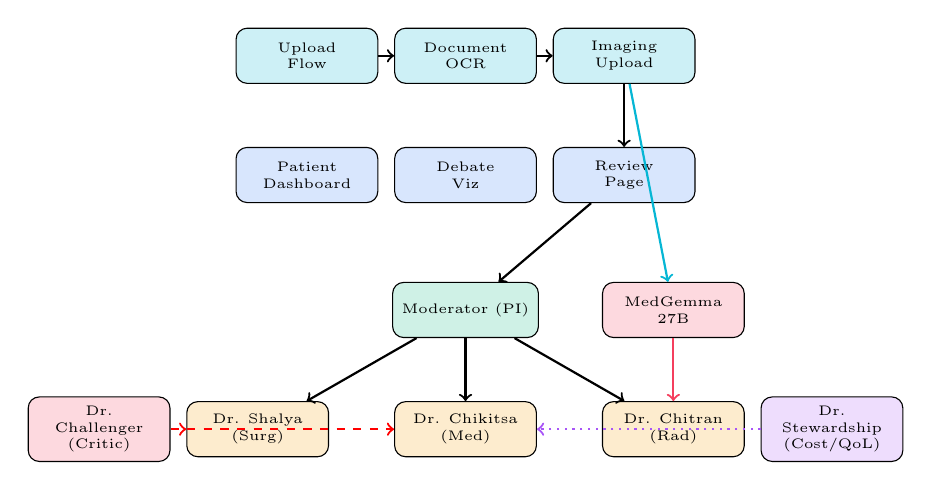
\begin{tikzpicture}[
    node distance=0.6cm,
    box/.style={rectangle, draw, rounded corners, minimum width=1.8cm, minimum height=0.7cm, align=center, font=\tiny},
    layer/.style={rectangle, draw, dashed, rounded corners},
    arrow/.style={->, thick}
]

% Upload Layer
\node[box, fill=cyan!20] (upload) {Upload\\Flow};
\node[box, fill=cyan!20, right=0.2cm of upload] (docs) {Document\\OCR};
\node[box, fill=cyan!20, right=0.2cm of docs] (imaging) {Imaging\\Upload};

% Presentation Layer
\node[box, fill=skyblue!20, below=0.8cm of upload] (ui) {Patient\\Dashboard};
\node[box, fill=skyblue!20, right=0.2cm of ui] (viz) {Debate\\Viz};
\node[box, fill=skyblue!20, right=0.2cm of viz] (review) {Review\\Page};

% Orchestration Layer
\node[box, fill=emerald!20, below=1cm of viz] (orch) {Moderator (PI)};

% Agents
\node[box, fill=amber!20, below left=0.8cm and 0.8cm of orch] (agent1) {Dr. Shalya\\(Surg)};
\node[box, fill=amber!20, below=0.8cm of orch] (agent2) {Dr. Chikitsa\\(Med)};
\node[box, fill=amber!20, below right=0.8cm and 0.8cm of orch] (agent3) {Dr. Chitran\\(Rad)};

% Control Agents
\node[box, fill=rose!20, left=0.2cm of agent1] (critic) {Dr.\\Challenger\\(Critic)};
\node[box, fill=purple!20, right=0.2cm of agent3] (steward) {Dr.\\Stewardship\\(Cost/QoL)};

% MedGemma
\node[box, fill=rose!20, right=0.8cm of orch] (medgemma) {MedGemma\\27B};

% Arrows
\draw[arrow] (upload) -- (docs);
\draw[arrow] (docs) -- (imaging);
\draw[arrow] (imaging) -- (review);
\draw[arrow, cyan] (imaging) -- (medgemma);
\draw[arrow] (review) -- (orch);
\draw[arrow] (orch) -- (agent1);
\draw[arrow] (orch) -- (agent2);
\draw[arrow] (orch) -- (agent3);
\draw[arrow, red, dashed] (critic) -- (agent1);
\draw[arrow, red, dashed] (critic) -- (agent2);
\draw[arrow, purple, dotted] (steward) -- (agent2);
\draw[arrow, rose] (medgemma) -- (agent3);

\end{tikzpicture}
\caption{V3 Architecture showing the "Virtual Lab" structure. Dr. Challenger and Dr. Stewardship provide lateral critique and constraints to the specialist agents.}
\label{fig:architecture}
\end{figure}

\section{Next-Gen Deliberation Engine}

\subsection{The "Virtual Tumor Board Lab" Structure}

We organize agents not as peers, but with distinct functional roles:

\begin{enumerate}[leftmargin=*]
    \item \textbf{The Moderator (PI)}: Sets the agenda, spawns parallel simulation threads if needed, and synthesizes the final consensus.
    \item \textbf{Clinical Specialists}: (Surgical, Medical, Radiation, Pathology, Genetics) - Generate hypotheses and treatment plans.
    \item \textbf{Dr. Challenger (The Scientific Critic)}: A dedicated adversarial agent that \textit{does not} propose treatments. Its sole function is to identify guideline violations (NCCN/ESMO), drug interactions, and safety risks. It acts as a check against hallucination.
    \item \textbf{Dr. Stewardship}: The financial and QoL watchdog. It weighs "Financial Toxicity" and patient values against marginal clinical benefits, asking "Is the 2-week survival benefit worth the bankruptcy risk?"
\end{enumerate}

\subsection{Chain of Debate Workflow}

Deliberation proceeds in four structured phases:

\subsubsection{Phase 1: The Information Gap (Gatekeeper)}
Before proposing plans, agents must identify missing data. The Moderator asks "What is missing?" If critical data (e.g., EGFR status) is absent, agents must explicitly state "Unknown" or recommend testing, rather than hallucinating values.

\subsubsection{Phase 2: Independent Hypothesis Generation}
To avoid anchoring bias, specialists generate their ideal plans in isolation (private chain-of-thought) before seeing others' opinions.

\subsubsection{Phase 3: The Adversarial Meeting}
\begin{itemize}
    \item \textbf{Round 1 (Proposals)}: Agents present independent plans.
    \item \textbf{Round 2 (Critique)}: \textbf{Dr. Challenger} critiques all plans for safety and guideline adherence. \textbf{Dr. Stewardship} flags cost/QoL concerns.
    \item \textbf{Round 3 (Rebuttal)}: Specialists update plans based on valid critiques.
\end{itemize}

\subsubsection{Phase 4: Conflict Resolution & Domain Veto}
If conflicts persist (e.g., Surgery vs. Neoadjuvant Chemo), the system applies \textbf{Domain Authority}:
\begin{itemize}
    \item \textbf{Surgical Oncologist} has Veto power on resectability.
    \item \textbf{Medical Oncologist} has Veto power on systemic therapy tolerance.
    \item \textbf{Radiologist} has Veto power on anatomical feasibility.
\end{itemize}

\section{Integrated Imaging (V8 Pipeline)}

\subsection{MedGemma Integration}
Our V8 pipeline integrates Google's MedGemma 27B model. Dr. Chitran (AI Radiologist) receives enhanced context from uploaded imaging:

\begin{enumerate}[leftmargin=*]
    \item \textbf{DICOM Upload}: Client-side parsing of CDs/DVDs.
    \item \textbf{Phone Capture}: Validated capture of X-ray films/prints.
    \item \textbf{AI Analysis}: MedGemma provides finding descriptions, measurements, and oncologic impressions.
\end{enumerate}

Dr. Chitran reconciles this AI analysis with uploaded text reports, flagging discrepancies (>20\% measurement difference) for the board.

\section{Implementation & Discussion}

The system is implemented in Next.js 15 with a multi-agent backend. Early testing suggests the adversarial model significantly reduces "agreeable hallucinations" where agents previously reinforced each other's errors. The explicit "Critic" role ensures safety checks are never skipped, while the "Stewardship" role brings essential developing-world economic reality into the clinical decision matrix.

\section{Conclusion}

The V3 Virtual Tumor Board represents a shift from passive "second opinion" chatbots to rigorous, adversarial clinical reasoning systems. By combining this with democratized imaging access via MedGemma, we provide a robust, safety-aware, and accessible oncology decision support tool.

\section*{Code Availability}
Source: \url{https://github.com/inventcures/virtual-tumor-board}

\end{document}
